\documentclass{article}
\usepackage[utf8]{inputenc}
\usepackage{babel}
\usepackage[a4paper, top = 20mm, bottom=20mm, right=20mm, left=20mm] {geometry}
\usepackage{graphicx}
\usepackage{amsmath}
\usepackage{wrapfig}
\usepackage{xcolor}
\usepackage[hidelinks]{hyperref}
\usepackage{listingsutf8}
\usepackage{tocloft}
\setlength{\parindent}{3mm}
\setlength{\parskip}{5mm}
\linespread{1.65}

\renewcommand{\figurename}{Fig.}
\renewcommand{\cftsecleader}{\cftdotfill{\cftdotsep}}
\newcommand{\seccion}[1]{
\hyperref[fig:toc]{\vspace{-2cm}\section{{#1}}\phantom{}\vspace{-1.5cm}}}
\newcommand{\subseccion}[1]{
\hyperref[fig:toc]{\vspace{-2cm}\subsection{{#1}}\phantom{}\vspace{-1.5cm}}}
\newcommand{\lstcaption}[1]{\hyperref[lsts]{{#1}}}
\newcommand{\figcaption}[1]{\caption[#1]{\hyperref[figs]{#1}}}

\lstset{
	language=Python,
	inputencoding=utf8/latin1,
	frame=single,
	numbers=left,
	basicstyle=\small\ttfamily, mathescape,
	numberstyle=\color{gray},
	stringstyle=\color[HTML]{933797},
	commentstyle=\color[HTML]{228B22}\sffamily,
	emph={[2]from,import,pass,return}, emphstyle={[2]\color[HTML]{DD52F0}},
	emph={[3]range}, emphstyle={[3]\color[HTML]{D17032}},
	emph={[4]for,in,def}, emphstyle={[4]\color{blue}},
	showstringspaces=false,
	breaklines=true,
	prebreak=\mbox{{\color{gray}\tiny$\searrow$}},
	captionpos=b,
}

\begin{document}
\title{\textbf{Sistemas de Información y Telemedicina.
\thanks{\href{https://www.upv.es/titulaciones/GIB/indexc.html}{Grado en Ingeniería Biomédica, Escuela Técnica Superior de Ingenieros Industriales, Valencia, España.}}}}
\date{\today}
\author{
\begin{tabular}{l@{\extracolsep{6em}}r}
\href{mailto:margisan@etsii.upv.es}{Marta Girones Sanguesa} &
\href{mailto:silmarg4@etsii.upv.es}{Silvia Marset Gomis}\\
\href{mailto:igamher@etsid.upv.es}{Ignacio Amat Hernández}&
\href{mailto:sogusan@etsii.upv.es}{Sofía Gutiérrez Santamaría}
\end{tabular}
}
\maketitle{}

\begin{figure}[h]
\tableofcontents{}
\addtocontents{toc}{\textbf{Sección}~\hfill\textbf{Página}\par}
\label{fig:toc}
\end{figure}

\newpage
\phantom{}
\vfill
\begin{figure}[h]
\phantomsection
\label{figs}
\listoffigures
\end{figure}
\vfill
\begin{figure}[h]
\phantomsection
\label{lsts}
\lstlistoflistings
\end{figure}
\vfill

\newpage

\phantom{}
\seccion{Preámbulo}
\vfill
\lstinputlisting[
	linerange = {8-38},
	caption = {[Importaciones iniciales y preparacion de datos.]
	\lstcaption{Importaciones iniciales y preparacion de datos.}},
	]{../python/src/preprocessing.py}
\vfill

\newpage
\seccion{Histogramas}

En este apartado dibujamos los histogramas comparativos.

\begin{figure}[h]
\centering
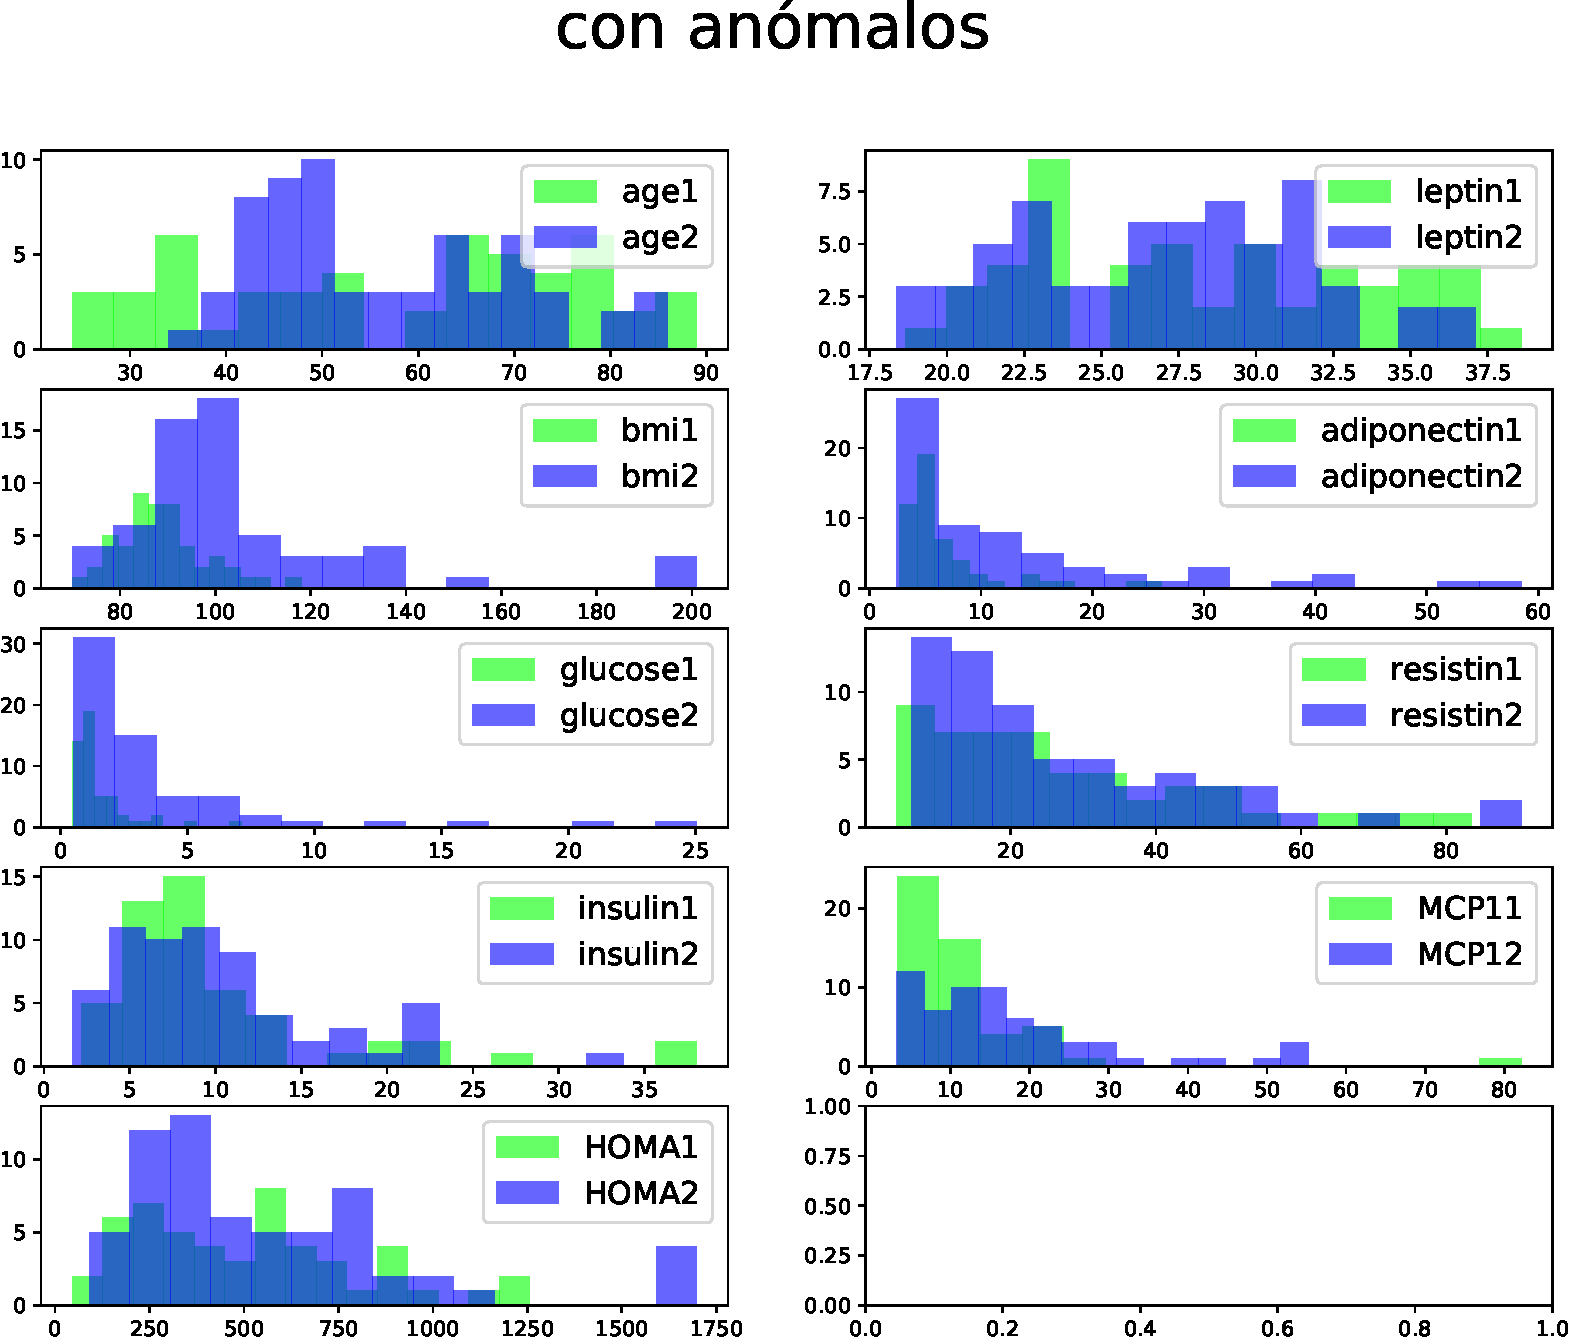
\includegraphics[width = 0.49\linewidth]{../python/images/hist.pdf}
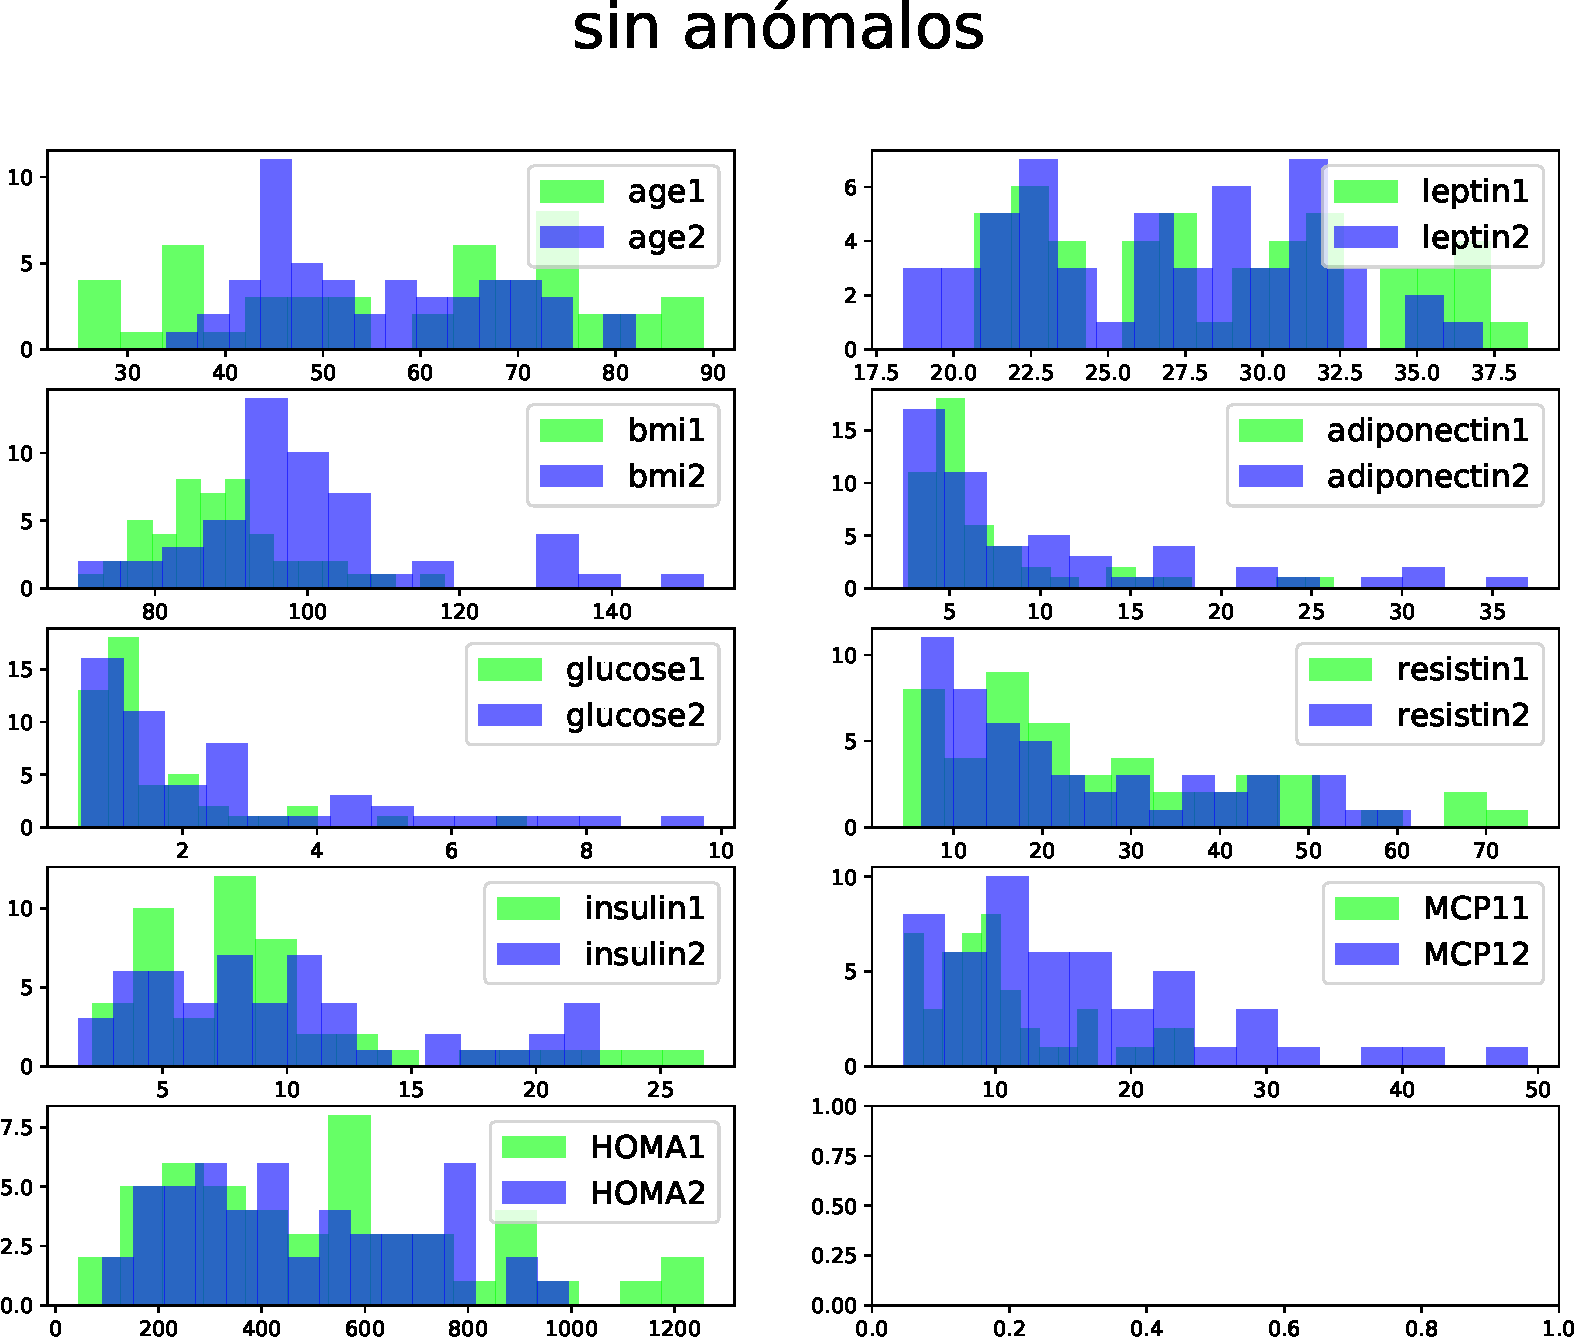
\includegraphics[width = 0.49\linewidth]{../python/images/hist1.pdf}
\figcaption{Histogramas para datos con y sin anomalias.}
\label{fig:hists}
\end{figure}

\lstinputlisting[
	linerange = {9-30},
	caption = {[C\'odigo generador de los histogramas con datos an\'omalos.]
	\lstcaption{C\'odigo generador de los histogramas con datos an\'omalos.}},
	]{../python/src/histograms.py}

\seccion{Kernel Density}

\begin{figure}[h]
\centering
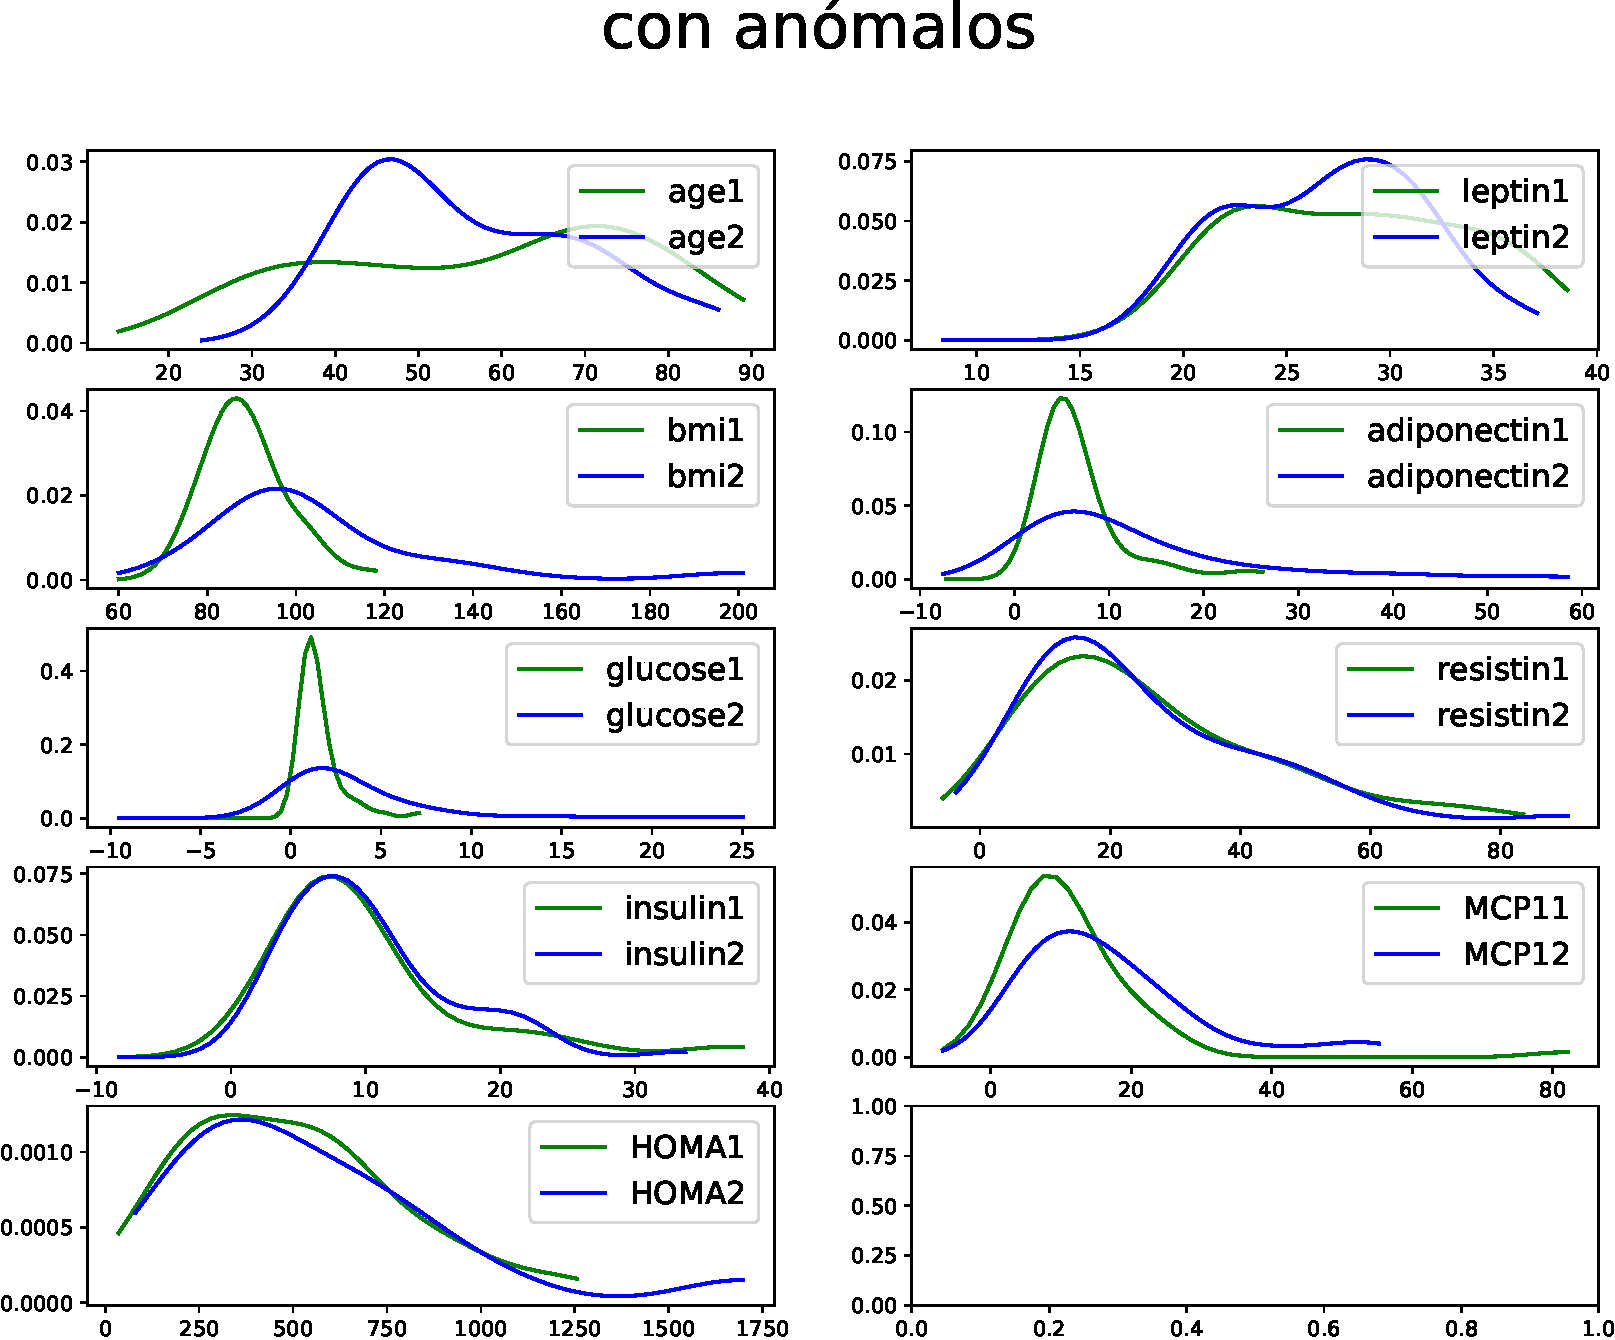
\includegraphics[width = 0.49\linewidth]{../python/images/kden.pdf}
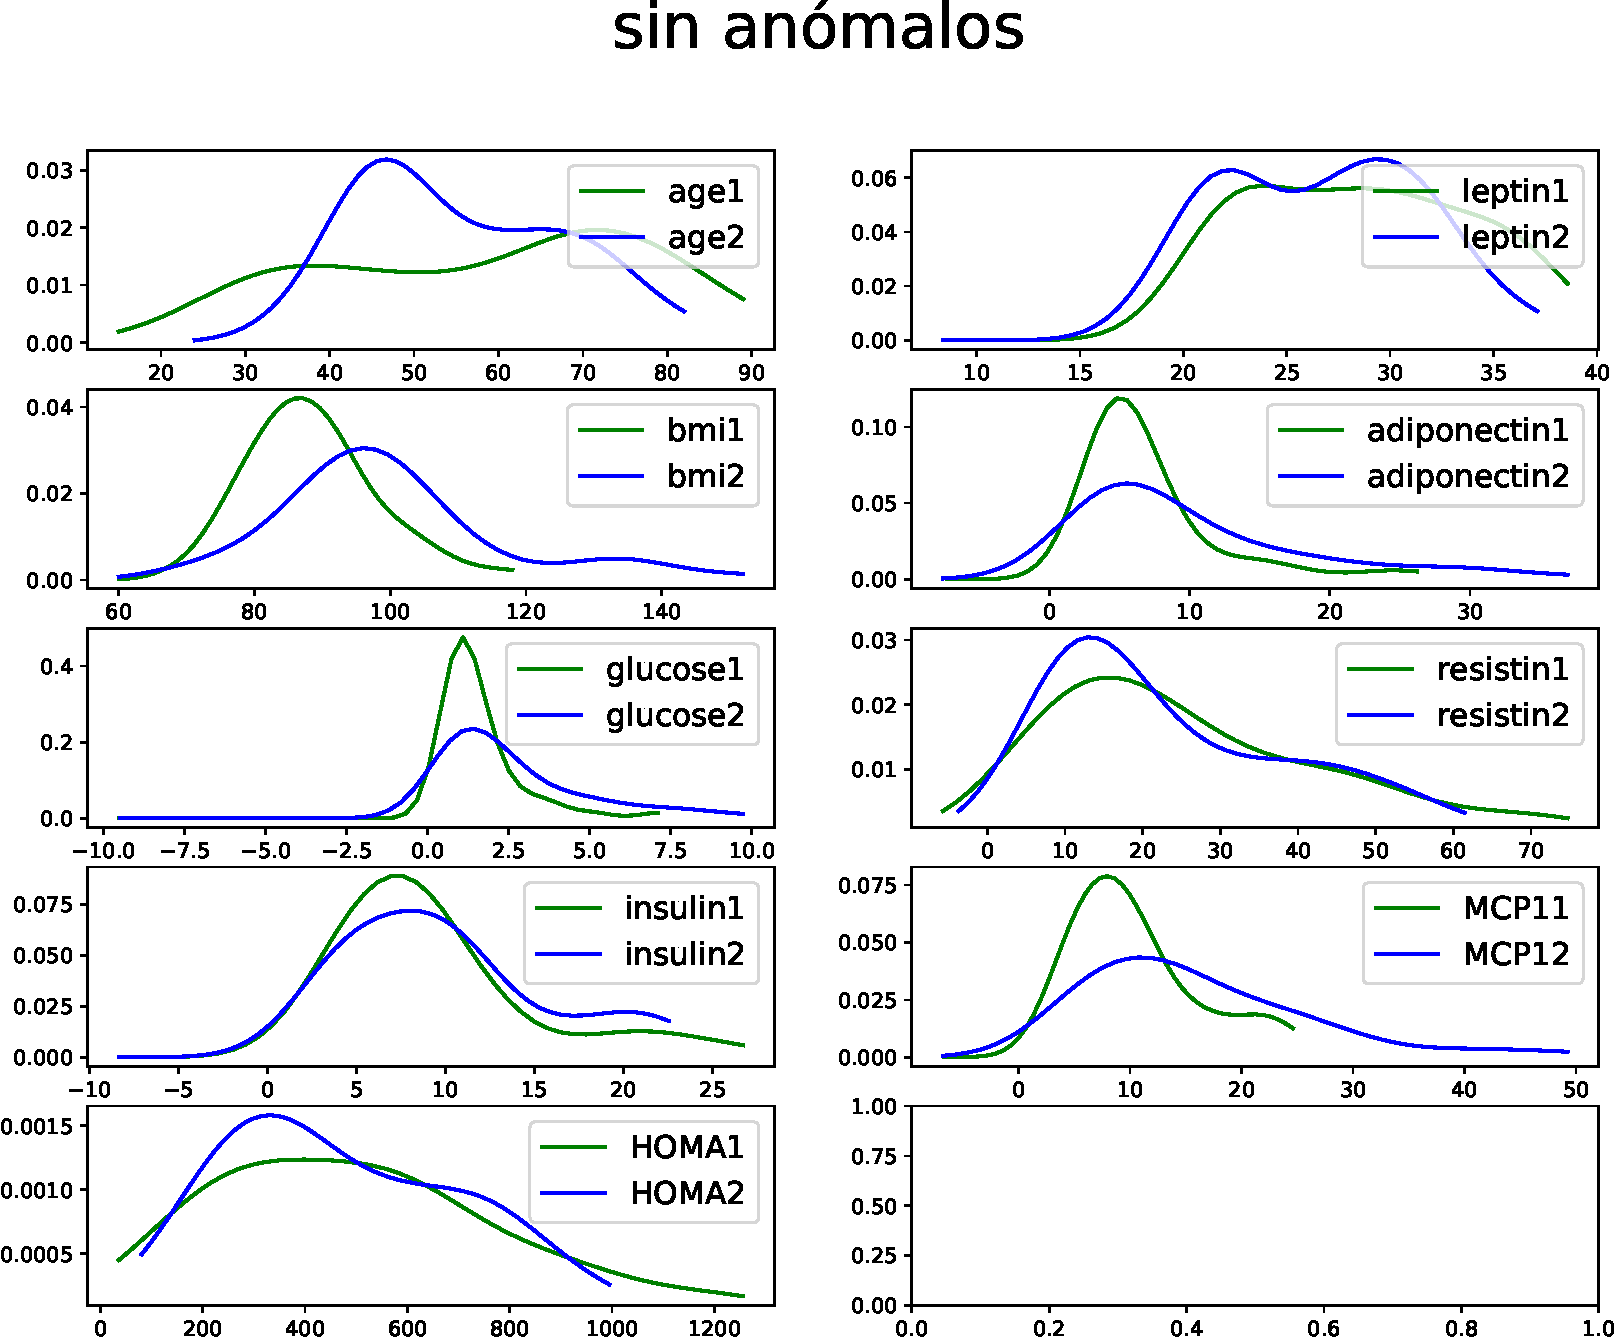
\includegraphics[width = 0.49\linewidth]{../python/images/kden1.pdf}
\figcaption{Kernel Density para datos con y sin anomalias.}
\label{fig:kdens}
\end{figure}

\lstinputlisting[
	linerange = {9-32},
	caption = {[C\'odigo generador de los kernel density plots con datos an\'omalos.]
	\lstcaption{C\'odigo generador de los kernel density plots con datos an\'omalos.}},
	]{../python/src/kerneldensity.py}

\seccion{Boxplot}

\begin{figure}[h]
\centering
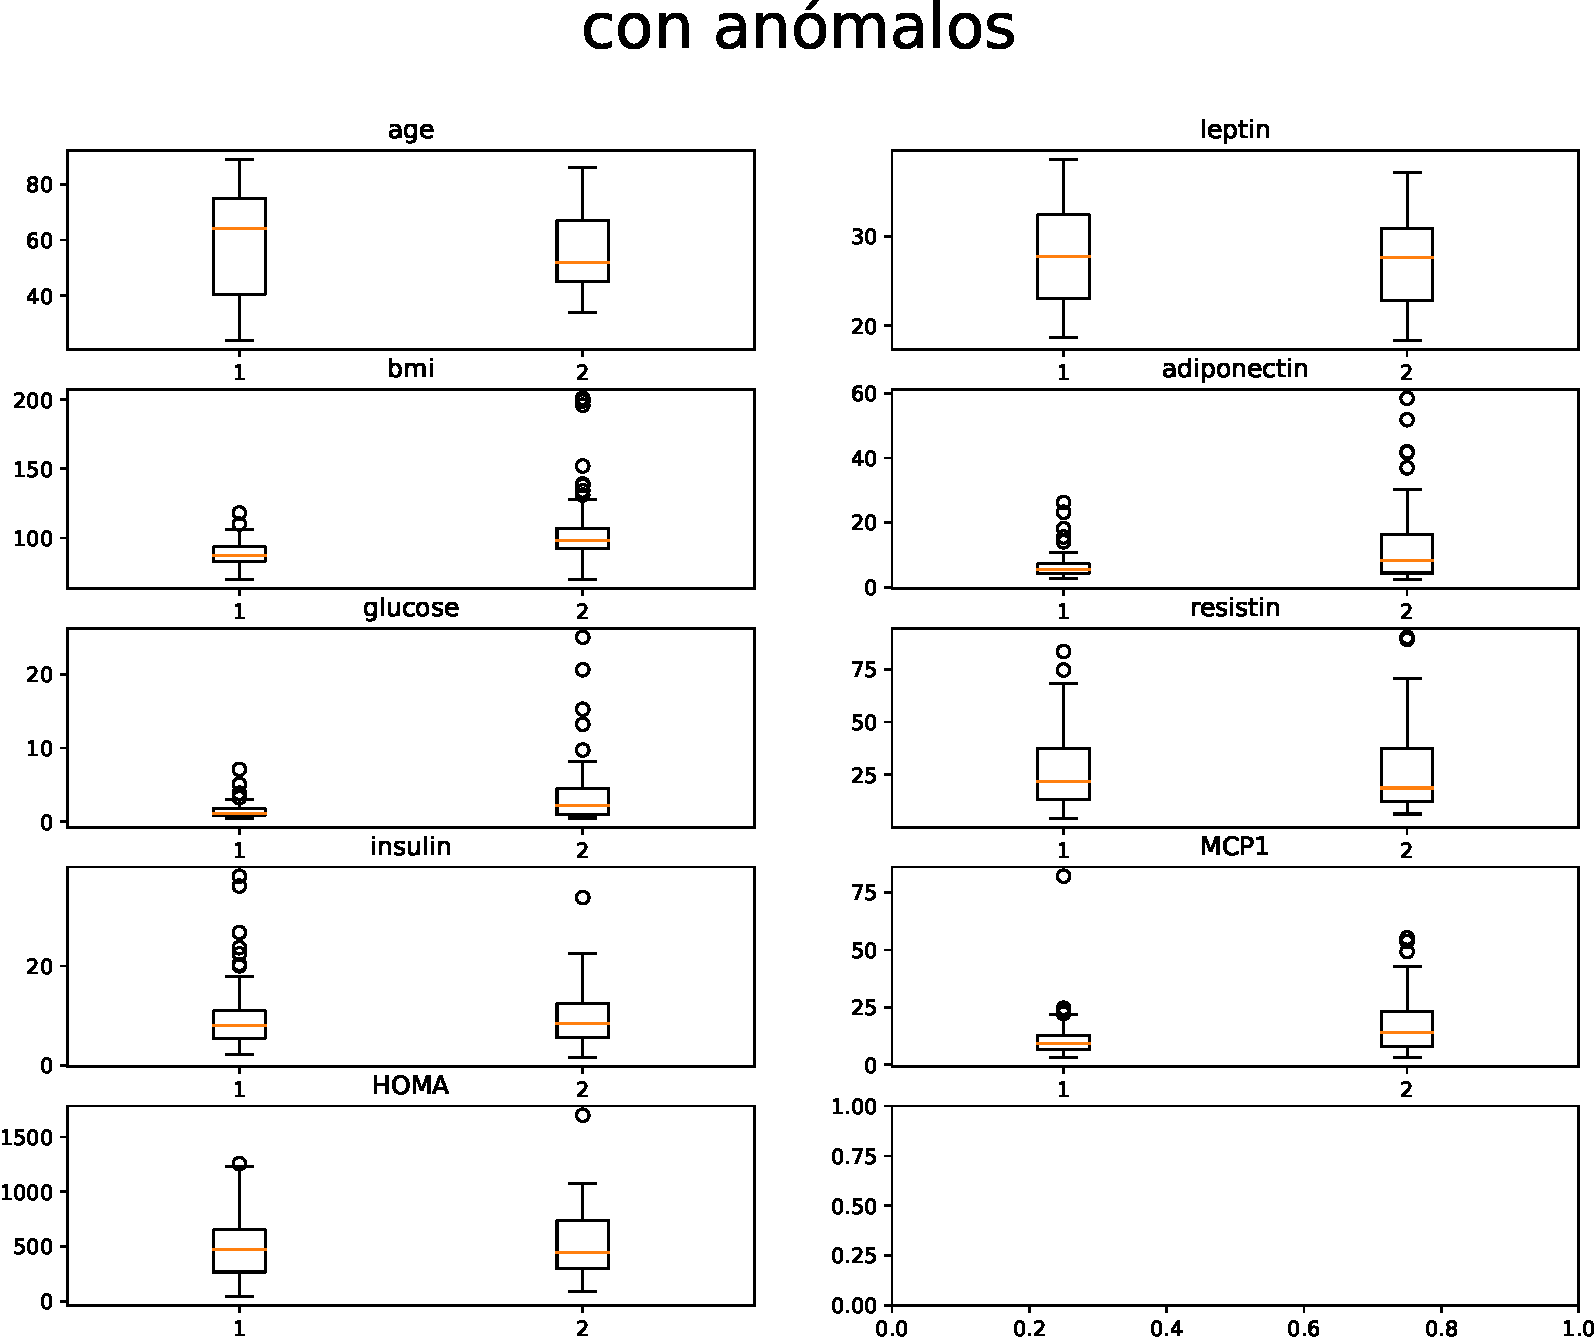
\includegraphics[width = 0.49\linewidth]{../python/images/boxp.pdf}
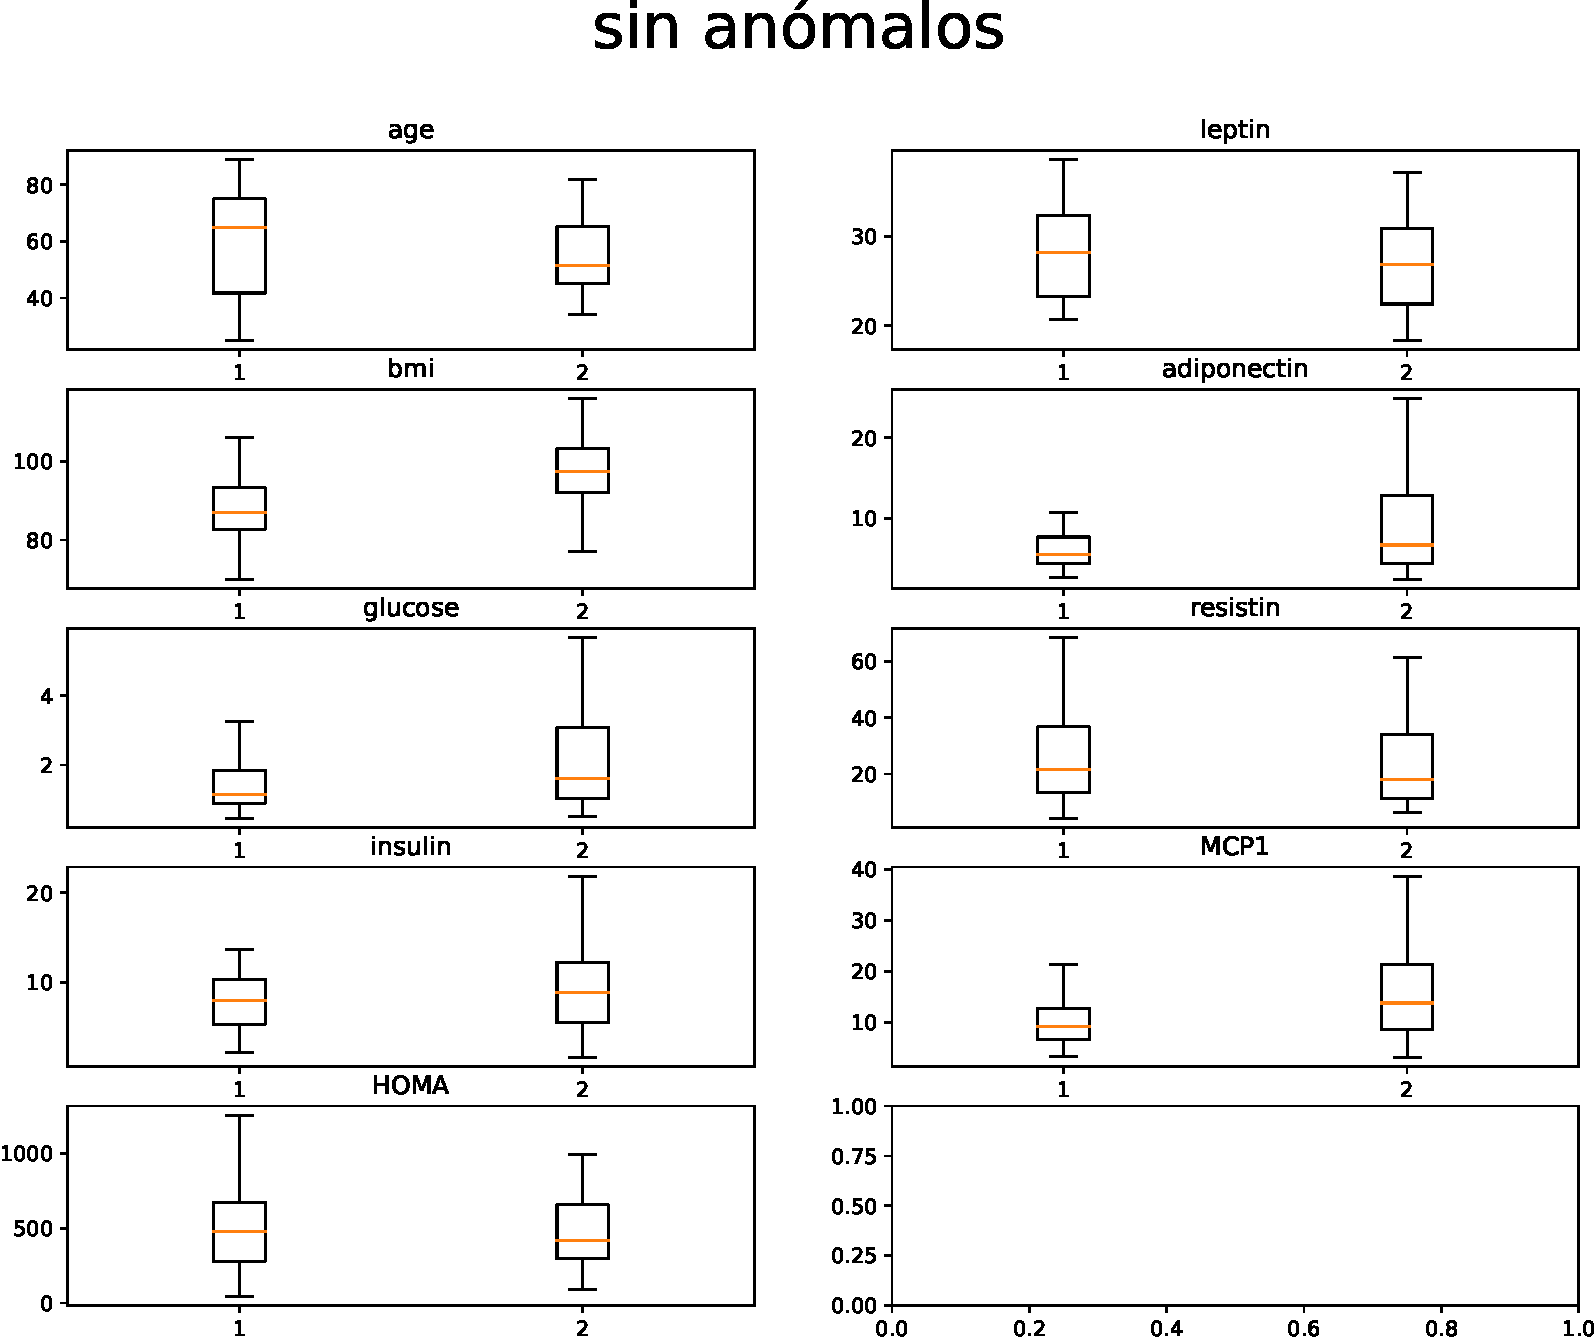
\includegraphics[width = 0.49\linewidth]{../python/images/boxp1.pdf}
\figcaption{Boxplots para datos con y sin anomalias.}
\label{fig:boxps}
\end{figure}

\lstinputlisting[
	linerange = {9-24},
	caption = {[C\'odigo generador de los boxplots con datos an\'omalos.]
	\lstcaption{C\'odigo generador de los boxplots con datos an\'omalos.}},
	]{../python/src/boxplot.py}

\newpage
\seccion{QQplot}

\begin{figure}[h]
\centering
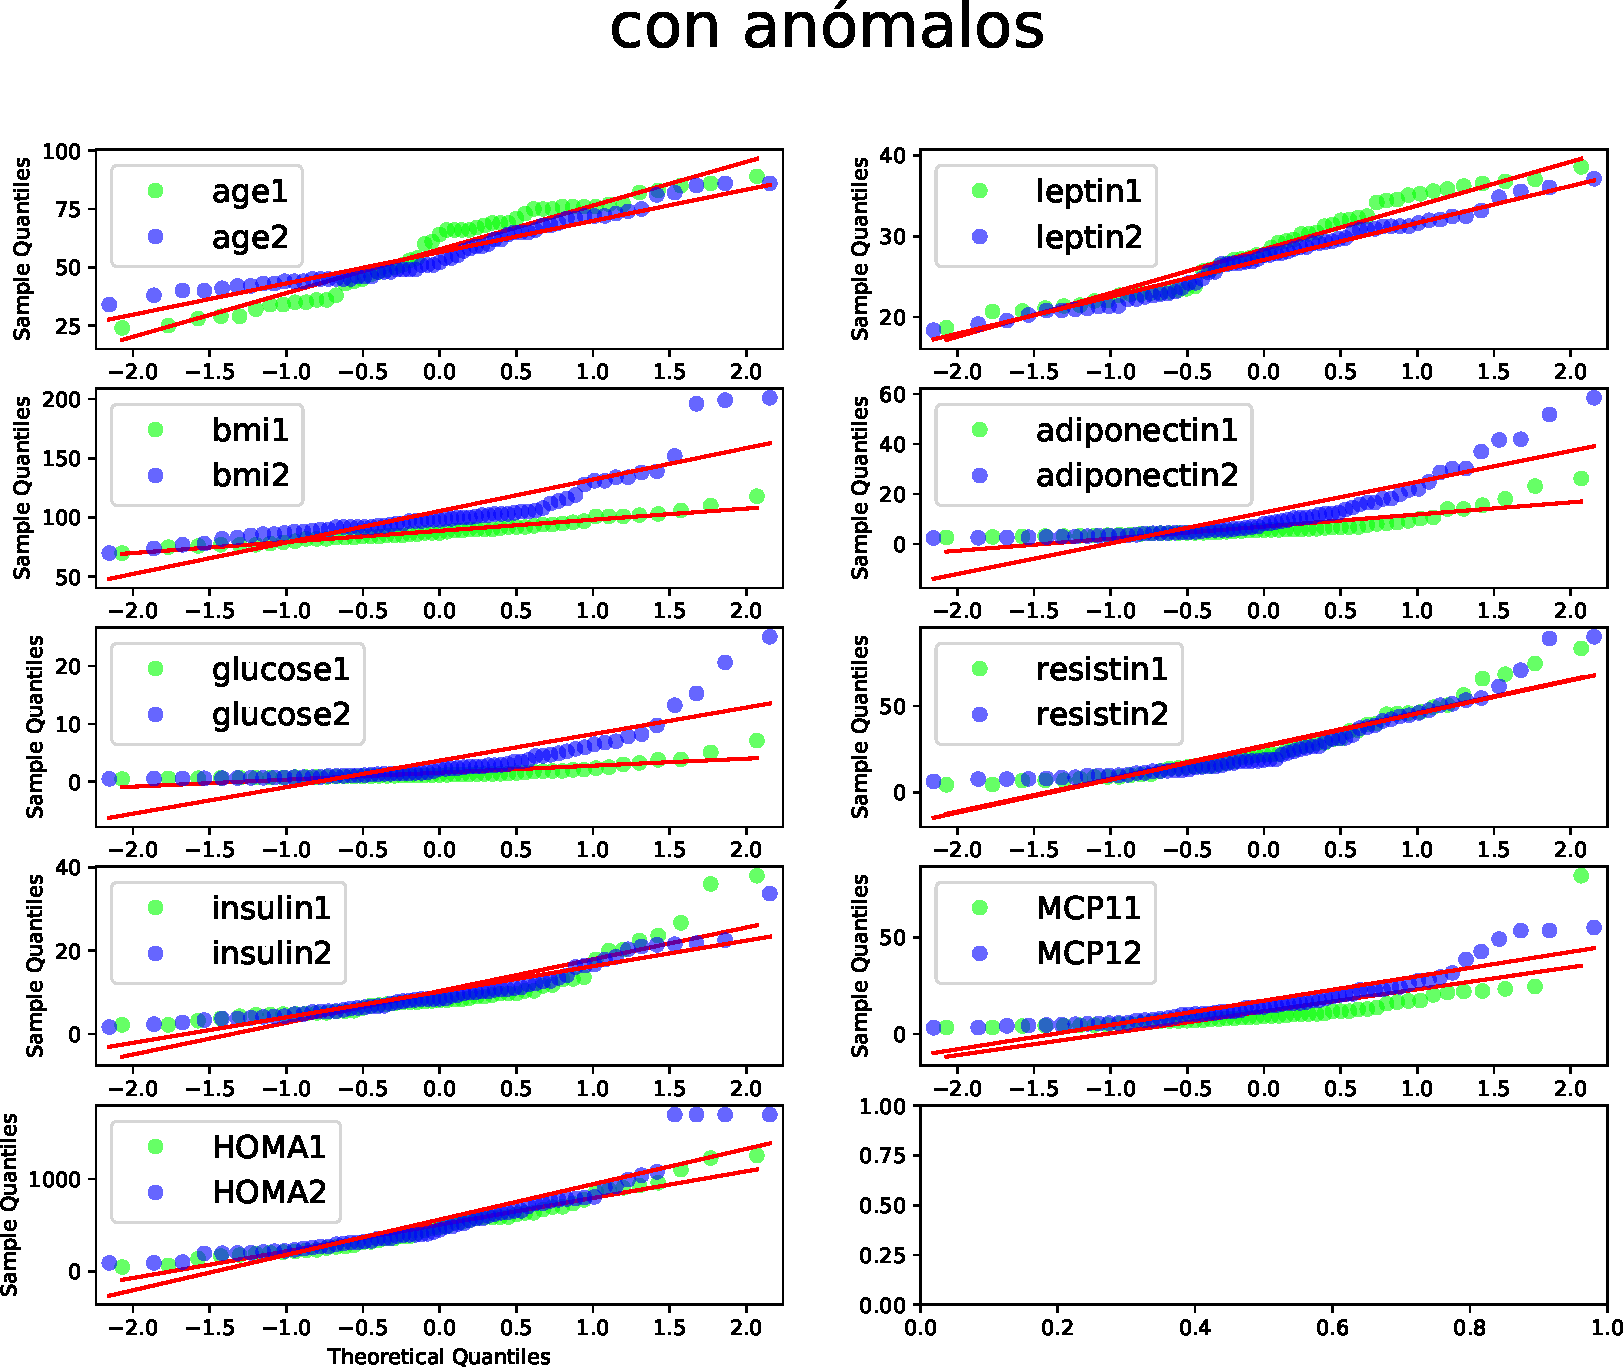
\includegraphics[width = 0.49\linewidth]{../python/images/qqp.pdf}
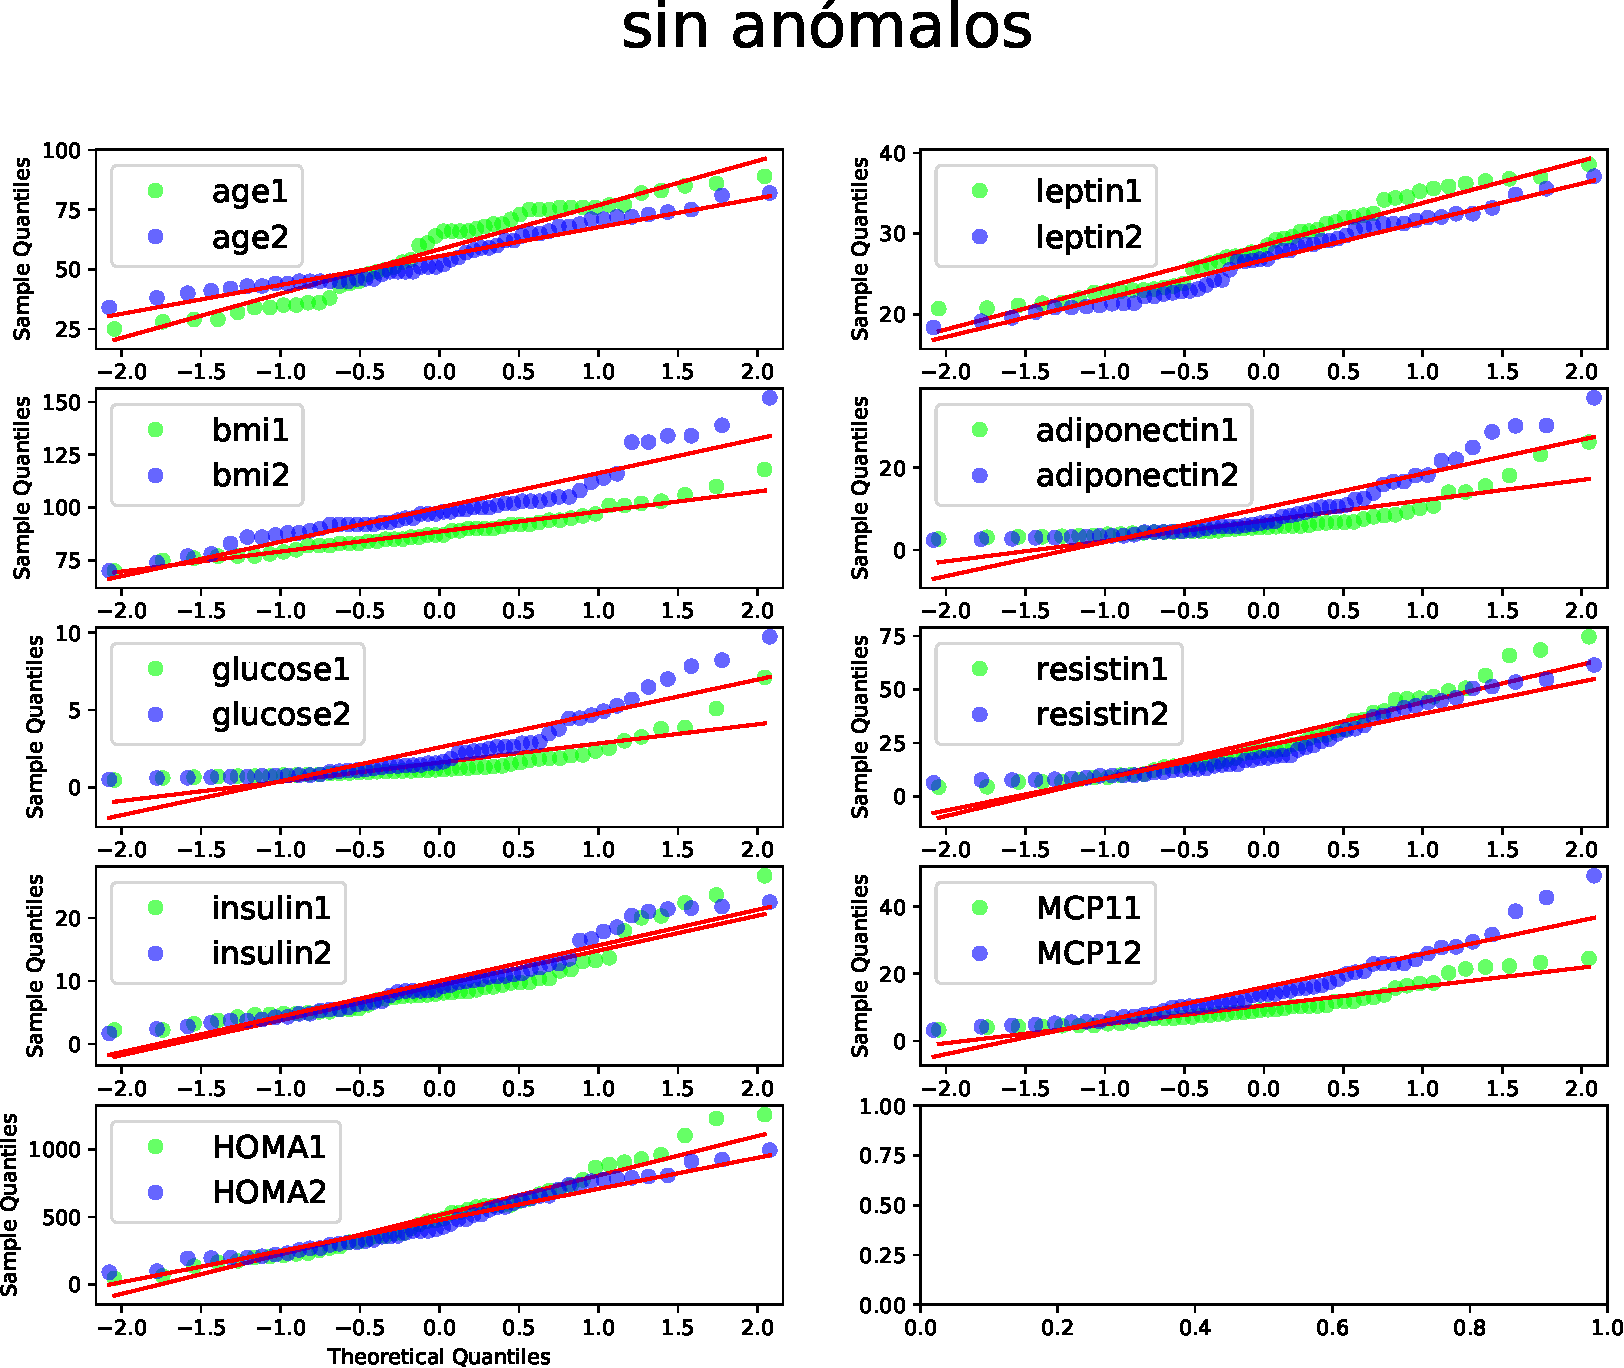
\includegraphics[width = 0.49\linewidth]{../python/images/qqp1.pdf}
\figcaption{QQplots para datos con y sin anomalias.}
\label{fig:qqps}
\end{figure}

\lstinputlisting[
	linerange = {9-28},
	caption = {[C\'odigo generador de los QQplots con datos an\'omalos.]
	\lstcaption{C\'odigo generador de los QQplots con datos an\'omalos.}},
	]{../python/src/qqplot.py}

\newpage
\seccion{Corrplot}
\vfill
\lstinputlisting[
	linerange = {13-17},
	caption = {[C\'odigo generador de los corrplots con datos an\'omalos.]
	\lstcaption{C\'odigo generador de los corrplots con datos an\'omalos.}},
	]{../python/src/corrplot.py}
\vfill
\begin{figure}[h]
\centering
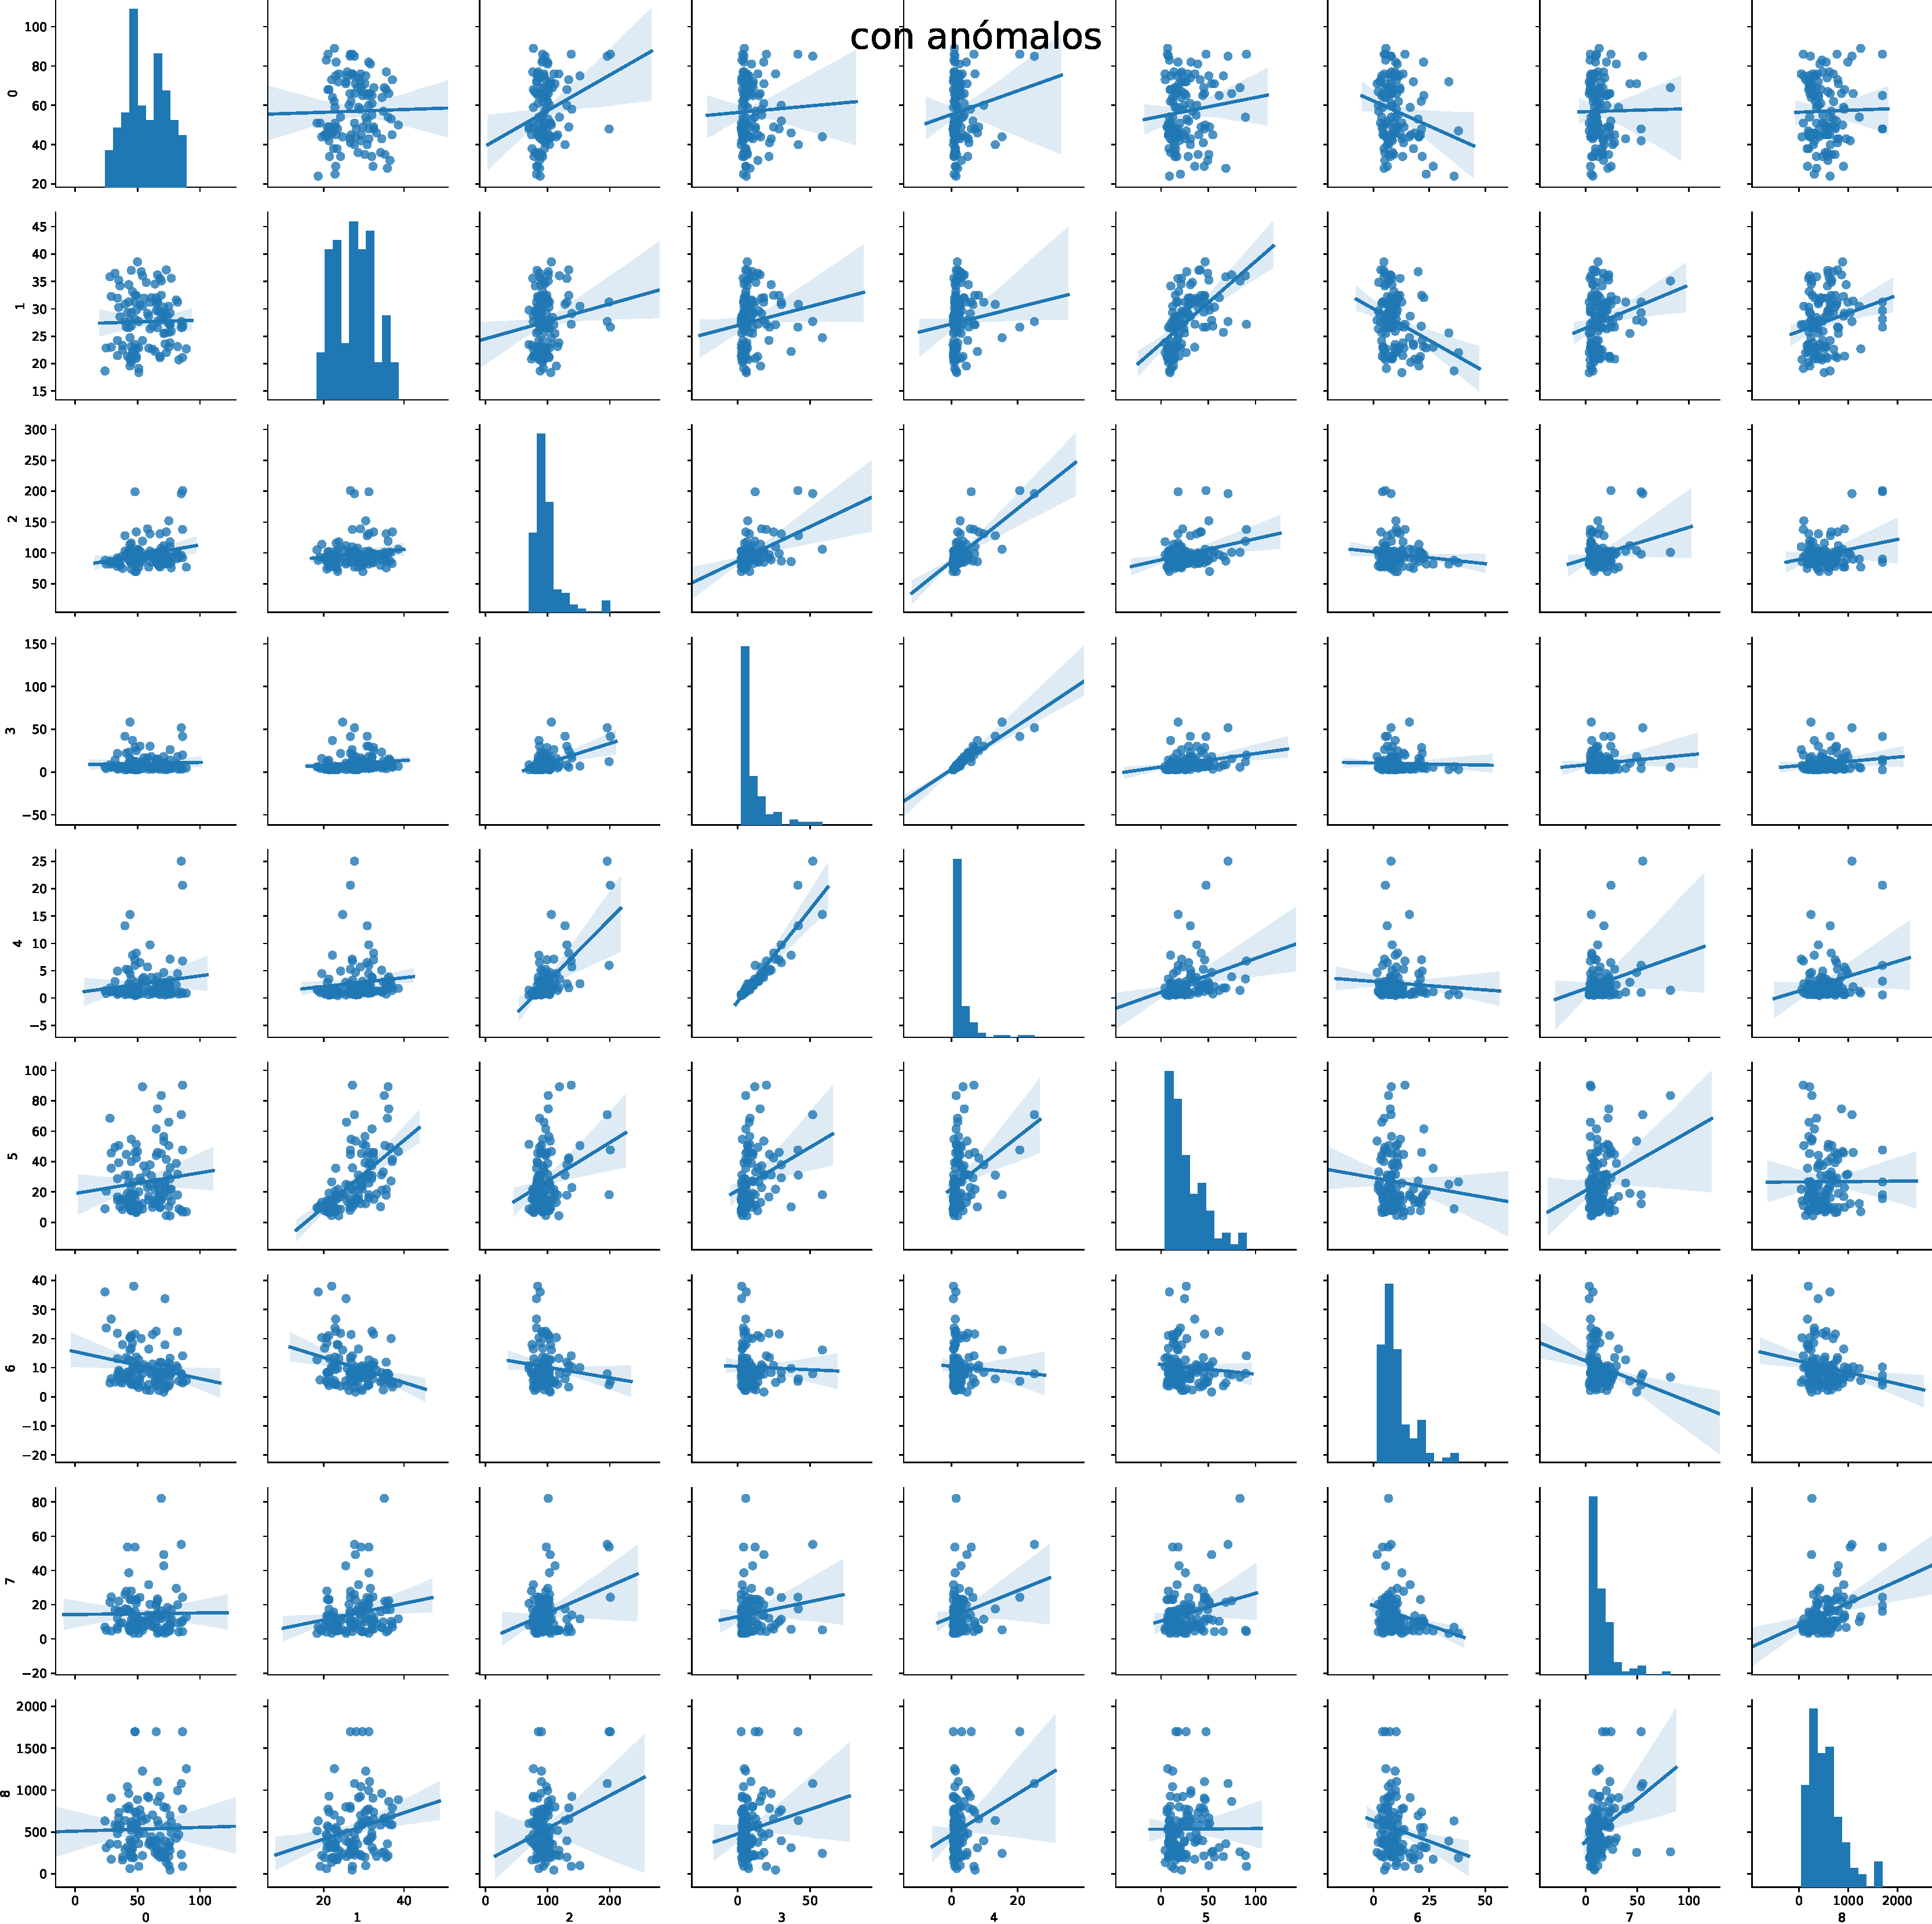
\includegraphics[width = \linewidth]{../python/images/corrp.pdf}
\figcaption{Corrplot para datos con anomalias.}
\label{fig:cps}
\end{figure}
\vfill

\newpage

\phantom{}
\vfill

\begin{figure}[h!]
\centering
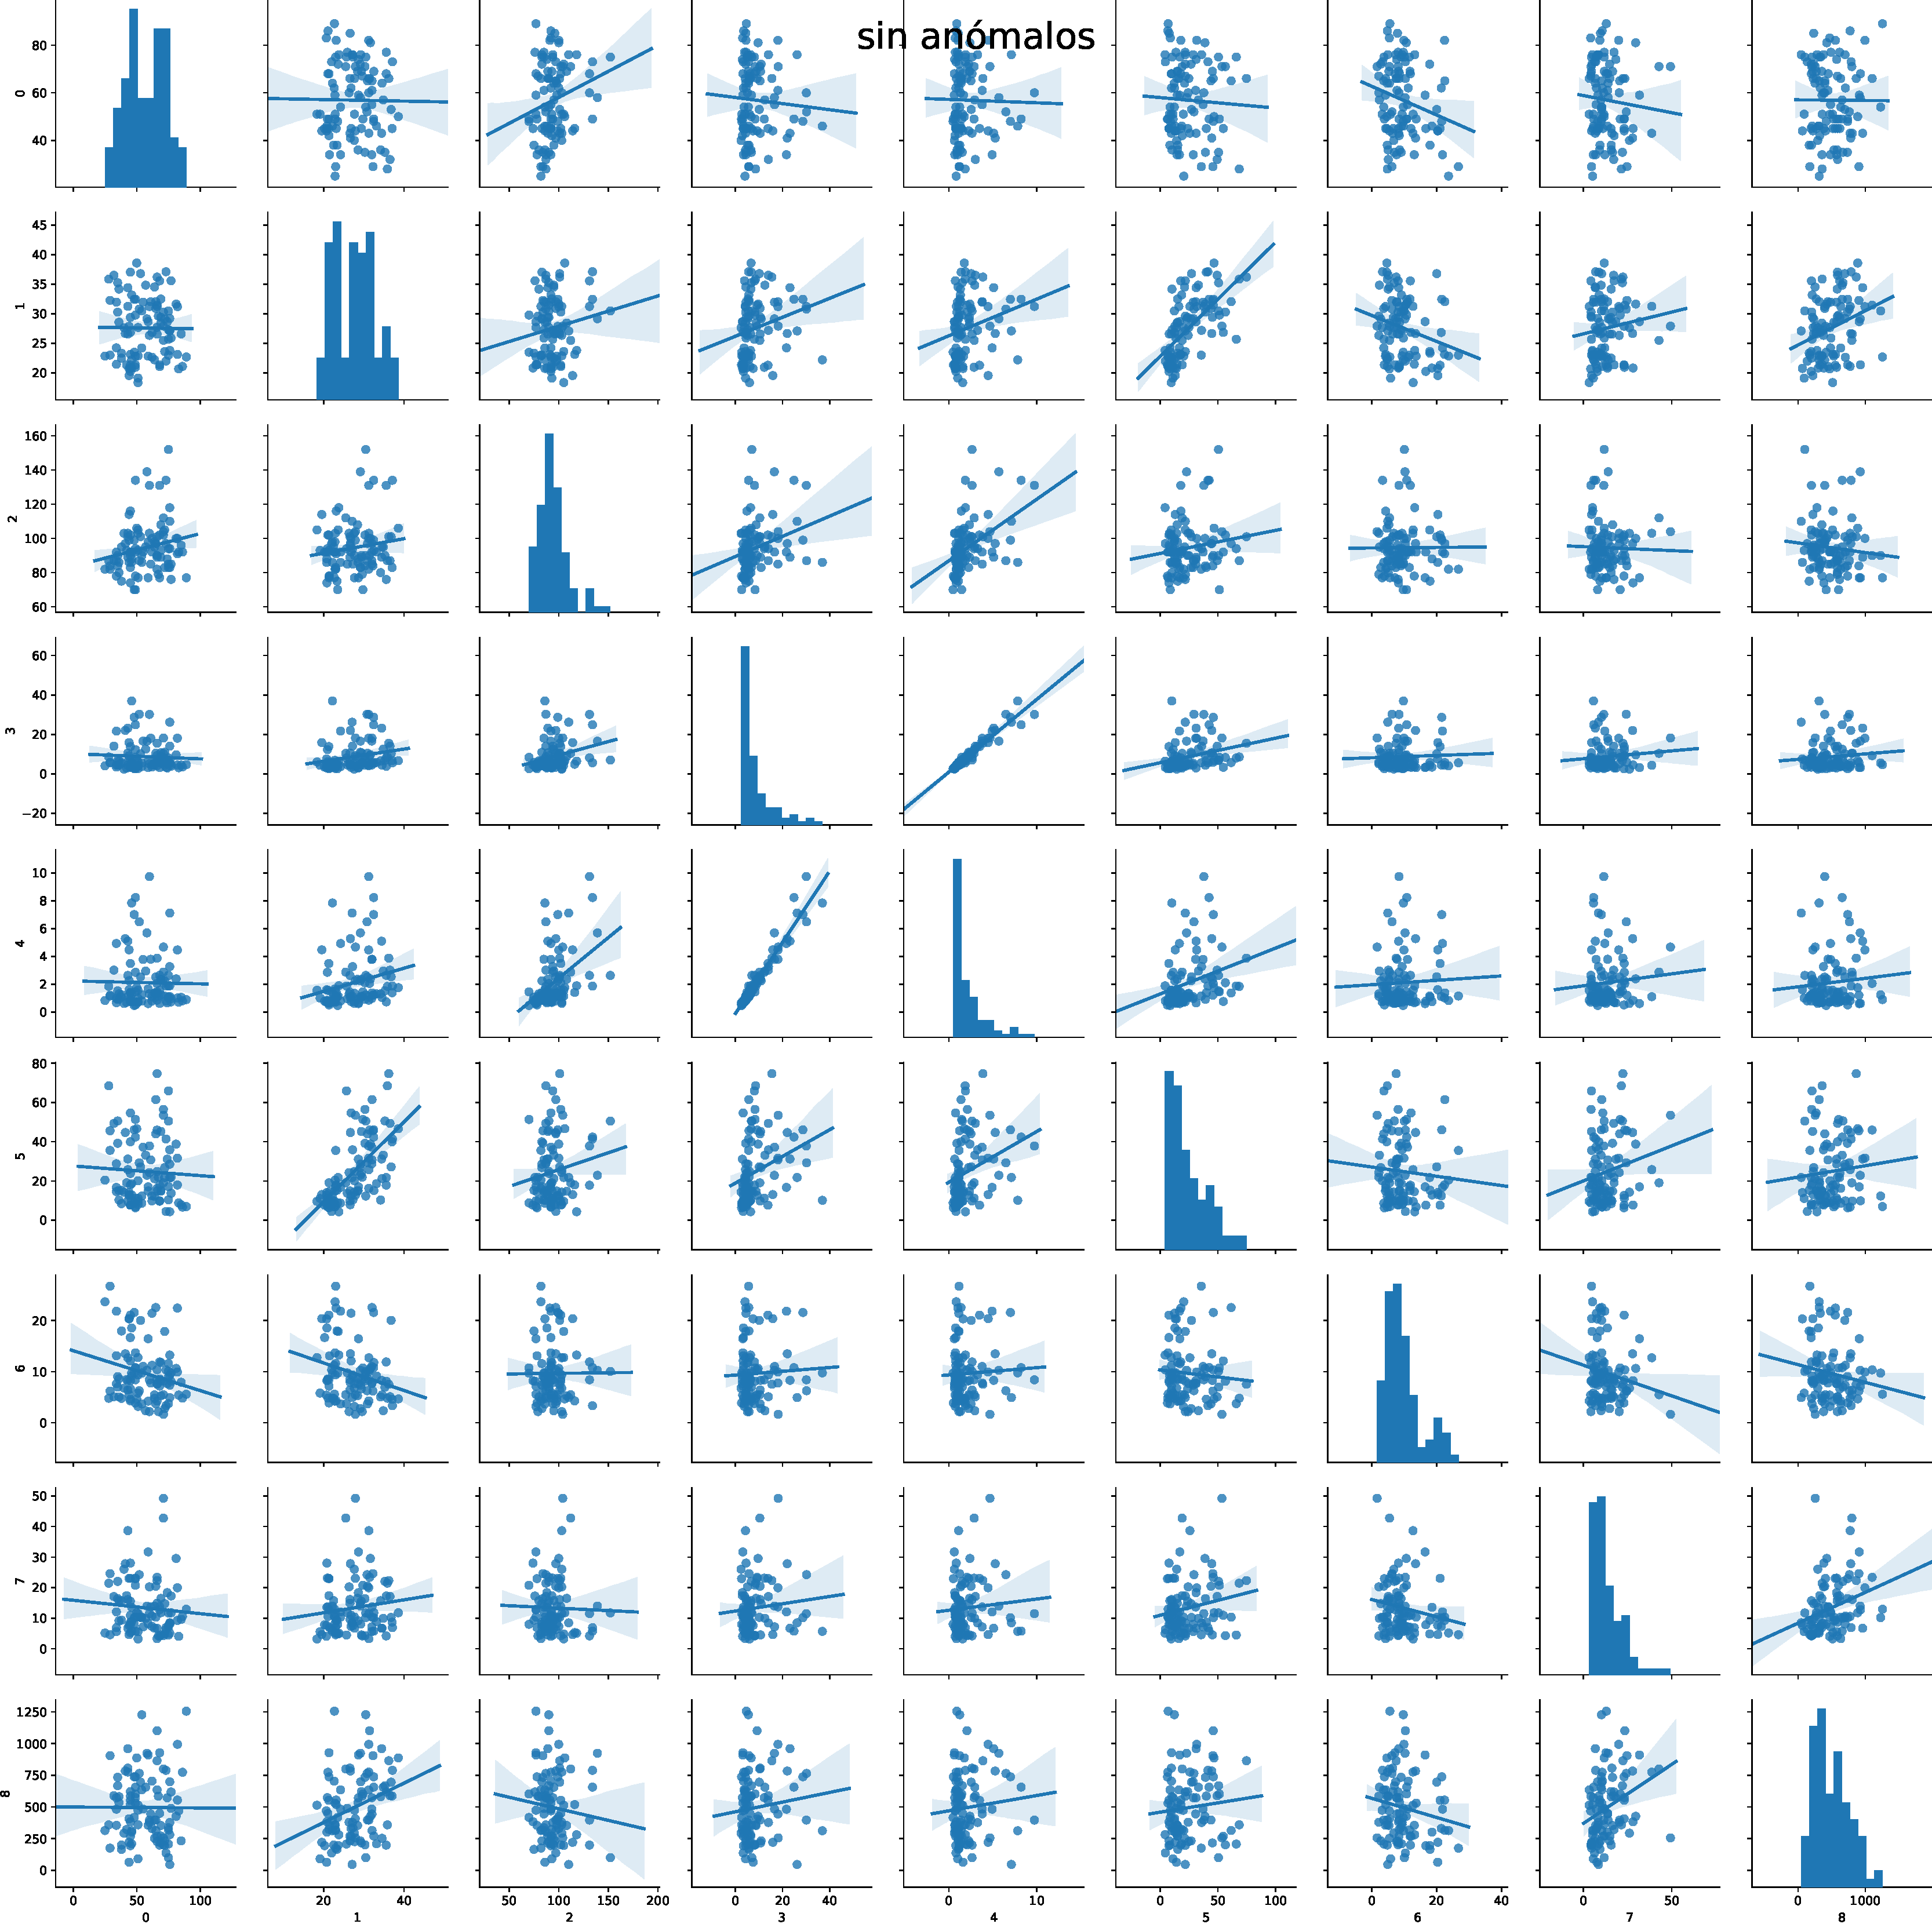
\includegraphics[width = \linewidth]{../python/images/corrp1.pdf}
\figcaption{Corrplot para datos sin anomalias.}
\label{fig:cp1s}
\end{figure}

\vfill

\newpage
\seccion{Filter Methods}

\lstinputlisting[
	linerange = {16 - 32},
	caption = {[Aplicaci\'on m\'etodos \textit{filter} de selecci\'on caracter\'isticas.]
	\lstcaption{Aplicaci\'on m\'etodos \textit{filter} de selecci\'on caracter\'isticas.}},
	]{../python/src/featureselection.py}

\begin{lstlisting}[
	caption = {[Ranking de variables seg\'un los m\'etodos filter.]
	{\lstcaption{Ranking de variables seg\'un los m\'etodos filter.}}},
	]
[4 5 9 6 7 3 1 8 2] -> fscore
[1 9 8 7 6 5 4 2 3] -> relieff
[3 4 1 1 1 2 3 6 1] -> diferencias
2.4444444444444446  -> media
\end{lstlisting}

\newpage
\seccion{Wrapper Methods}

\lstinputlisting[
	linerange = {37 - 58},
	caption = {[Aplicaci\'on m\'etodos \textit{wrapper} de selecci\'on caracter\'isticas.]
	\lstcaption{Aplicaci\'on m\'etodos \textit{wrapper} de selecci\'on caracter\'isticas.}},
	]{../python/src/featureselection.py}

\begin{lstlisting}[
	caption = { [Resultados del filtrado mediante wrappers.]
	{\lstcaption{Resultados del filtrado mediante wrappers.}}},
	]
0.7054545454545454
Sequential Forward  Selection ('leptin', 'bmi', 'glucose', 'MCP1')

0.7094949494949495
Sequential Backward Selection ('leptin', 'bmi', 'glucose', 'insulin')
\end{lstlisting}
\newpage
\seccion{PCA}

\lstinputlisting[
	linerange = {60-67},
	caption = {[\textit{Principal Component Analysis}]
	\lstcaption{\textit{Principal Component Analysis}}},
	]{../python/src/featureselection.py}

\subseccion{Pareto}

\begin{figure}[h]
\centering
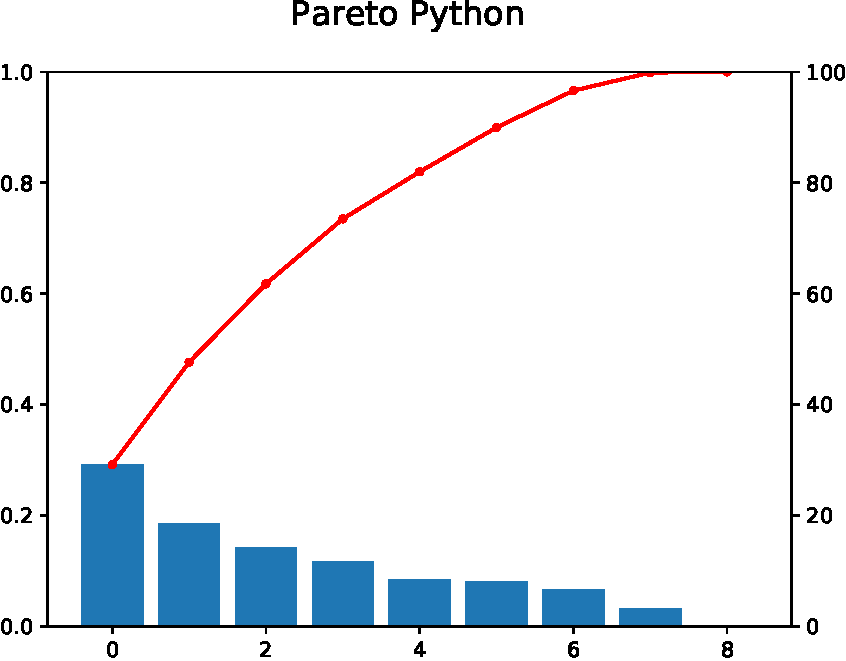
\includegraphics[width = 0.7\linewidth]{../python/images/pareto.pdf}
\figcaption{Diagrama de Pareto.}
\label{fig:pareto}
\end{figure}

\lstinputlisting[
	linerange = {72-82},
	caption = {[C\'odigo generador del diagrama de Pareto]
	\lstcaption{C\'odigo generador del diagrama de Pareto}},
	]{../python/src/featureselection.py}

\end{document}
